\documentclass[11pt,oneside]{book}
\usepackage[a4paper,top=24mm,bottom=25mm,inner=28mm,outer=24mm]{geometry}
\usepackage{fontspec}
\setmainfont{DejaVu Serif}
\setsansfont{DejaVu Sans}
\setmonofont{DejaVu Sans Mono}[Scale=0.88]
\usepackage{microtype}\n\emergencystretch=1.5em
\usepackage{amsmath,amssymb,mathtools}
\usepackage{booktabs,longtable,array,tabularx,multirow}
\usepackage{graphicx}
\usepackage{xcolor}
\definecolor{DNCblue}{HTML}{173B57}
\definecolor{DNCcyan}{HTML}{2B7A78}
\definecolor{DNCgold}{HTML}{B98936}
\definecolor{DNCink}{HTML}{17212B}
\definecolor{DNClight}{HTML}{F3F6F8}
\definecolor{DNCred}{HTML}{A23B3B}
\usepackage{tikz}
\usetikzlibrary{arrows.meta,positioning,calc,fit,shapes.geometric,backgrounds}
\usepackage{pgfplots}
\pgfplotsset{compat=1.18}
\usepackage[most]{tcolorbox}
\usepackage{listings}
\lstset{basicstyle=\ttfamily\footnotesize,breaklines=true,frame=single,rulecolor=\color{DNCblue!25},backgroundcolor=\color{DNClight},showstringspaces=false}
\usepackage{enumitem}
\setlist{nosep,leftmargin=1.6em}
\usepackage{fancyhdr}
\pagestyle{fancy}\fancyhf{}
\fancyhead[L]{\sffamily\small DNCrypt Monograph}\fancyhead[R]{\sffamily\small \leftmark}\fancyfoot[C]{\thepage}
\renewcommand{\headrulewidth}{0.3pt}
\usepackage{titlesec}
\titleformat{\chapter}[display]{\sffamily\bfseries\color{DNCblue}\raggedright}{\Large CHAPTER \thechapter}{6pt}{\Huge}
\titleformat{\section}{\sffamily\Large\bfseries\color{DNCblue}}{\thesection}{0.7em}{}
\titleformat{\subsection}{\sffamily\large\bfseries\color{DNCcyan}}{\thesubsection}{0.7em}{}
\usepackage{hyperref}
\hypersetup{colorlinks=true,linkcolor=DNCblue,citecolor=DNCcyan,urlcolor=DNCcyan,pdftitle={DNCrypt Monograph},pdfauthor={Adrian Lipa}}
\newtcolorbox{resultbox}[1][]{enhanced,breakable,colback=DNClight,colframe=DNCblue,boxrule=0.8pt,arc=2mm,title=#1,fonttitle=\sffamily\bfseries}
\newtcolorbox{evidencebox}[1][]{enhanced,breakable,colback=DNCcyan!5,colframe=DNCcyan,boxrule=0.8pt,arc=2mm,title=#1,fonttitle=\sffamily\bfseries}
\newtcolorbox{warningbox}[1][]{enhanced,breakable,colback=DNCred!4,colframe=DNCred,boxrule=0.8pt,arc=2mm,title=#1,fonttitle=\sffamily\bfseries}
\newcommand{\Hmin}{H_{\min}}
\newcommand{\Dn}{\textsf{DNCrypt}}
\newcommand{\code}[1]{\texttt{#1}}
\begin{document}
\frontmatter
\begin{titlepage}
\pagecolor{DNCink}\color{white}
\vspace*{18mm}
{\sffamily\bfseries\fontsize{42}{46}\selectfont DNCrypt\par}
\vspace{5mm}
{\sffamily\fontsize{19}{24}\selectfont Dynamic Noncommutative Cryptography\par}
\vspace{4mm}
{\sffamily\fontsize{15}{20}\selectfont A Provenance-Preserving Adaptive AEAD Architecture\\with Phase-Derived Entropy and 36D Information Topology\par}
\vfill
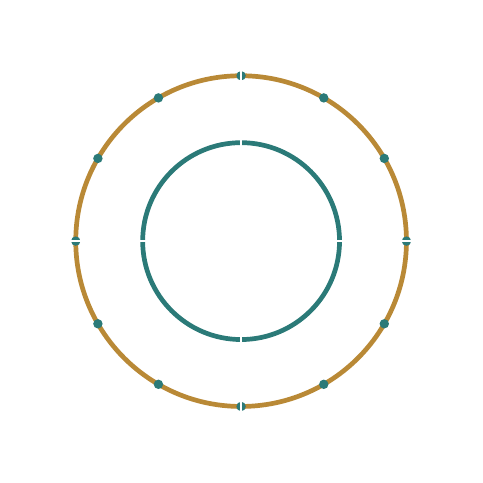
\begin{tikzpicture}[x=1cm,y=1cm]
  \draw[DNCcyan,line width=1.7pt] (0,0) circle (1.25);
  \draw[DNCgold,line width=1.7pt] (0,0) circle (2.10);
  \foreach \a in {0,30,...,330}{\fill[DNCcyan] ({2.1*cos(\a)},{2.1*sin(\a)}) circle (1.7pt);}
  \draw[white!65,line width=.6pt] (-2.7,0)--(2.7,0);
  \draw[white!65,line width=.6pt] (0,-2.7)--(0,2.7);
  \node[white,font=\sffamily\bfseries] at (0,0) {$T^{36}$};
\end{tikzpicture}
\vfill
{\sffamily\large Adrian Lipa\par}
\vspace{2mm}
{\sffamily\small Version 0.3 Research Monograph --- 24 August 2026\par}
\vspace{8mm}
{\sffamily\footnotesize Evidence status: IMPLEMENTATION CONFORMANCE PROTOTYPE\\[1mm]+ CONTROLLED SOFTWARE CRYPTANALYSIS BENCHMARK\par}
\end{titlepage}
\nopagecolor\color{DNCink}

\chapter*{Abstract}
\addcontentsline{toc}{chapter}{Abstract}
\Dn{} is an adaptive authenticated-encryption research architecture that combines a frozen standard cryptographic anchor with a mutable 36-dimensional public genome, a persistent cipher surface, append-only provenance, adversarial evaluation, and fail-closed evolutionary promotion. The current implementation anchors message confidentiality and integrity in ChaCha20-Poly1305, derives per-message keys through HKDF-SHA3-512, and binds genome generation, surface commitment, internal tick, lineage, and user associated data into authenticated metadata.

The present revision adds a native cryptographic algebra, a phase-derived entropy candidate based on the two-sheet relation between $4\pi$ and $2\pi$ phase descriptions, empirical min-entropy health gating, and a 36D entropy-topology selector based on per-coordinate min-entropy, pairwise mutual information, and cross-coordinate predictability. A controlled cryptanalysis benchmark compares a frozen static anchor against the adaptive loop under equal attack budgets using an independent train/holdout split. In the reference run, the adaptive variant won 4 of 12 holdout comparisons and the static anchor won 8 of 12, with a two-sided sign-test value $p=0.3877$. The benchmark therefore records the verdict \code{NO\_HOLDOUT\_ADVANTAGE\_DEMONSTRATED} and exposes selection generalization as the next experimental gate.

This monograph specifies the architecture, equations, evidence, benchmark protocol, reproducibility requirements, and next validation gates in one citable document.

\begin{evidencebox}[Repository evidence snapshot]
Repository: \code{AdrianLipa90/DNCrypt}. The repository migration audit is PASS. The repository-layout test suite after addition of the challenge contains 54 passing tests. GitHub status checks were not configured for the referenced commit series; repository evidence therefore separates local harness status from external CI status.
\end{evidencebox}

\tableofcontents
\listoffigures
\listoftables

\mainmatter
\chapter{Scope and Design Objective}
\section{System objective}
The system protects arbitrary application payloads while retaining an auditable, evolving public state. The security anchor is held fixed by protocol while the experimental outer state may mutate under bounded adversarial feedback. The architectural separation is
\begin{equation}
\boxed{\text{frozen AEAD/KDF anchor}}\quad\oplus\quad\boxed{\text{adaptive public genome and surface}}.
\end{equation}
The mutation authority is constrained to the public experimental state. Promotion is conditioned on decrypt and integrity invariants, exact evaluation coverage, Pareto survival, minimum risk improvement, and throughput retention.

\section{Evidence classes}
The repository currently contains three complementary evidence classes:
\begin{enumerate}
\item implementation conformance against standard cryptographic vectors;
\item live phase-entropy and 36D topology receipts from endogenous runtime dynamics;